%#################### 4.1 ####################
\section{Nice tcolorbox}
\begin{table}[h!]
\begin{tabular}{c | c}
\begin{minipage}[m]{0.4\textwidth}
\enum{
\begin{tcolorbox}[colback=white!100,colframe=red!75!black,width=7cm,righttitle=0.5cm,subtitle style={boxrule=0.4pt, colback=yellow!50!red!25!white},title= \bf{1}\hfill  \bf{22}]
	\begin{center}\bf{333}\end{center}
	\tcblower
	\href{https://tools.ietf.org/doc/texlive-doc/latex/tcolorbox/tcolorbox.pdf}{Source}
	\end{tcolorbox}}{4.1}
\end{minipage}
&
\begin{minipage}[m]{0.55\textwidth}
\renewcommand\textminus{\mbox{-}}%<<<<<<<<<<<
\begin{lstlisting}[numberstyle=\zebra{green!15}{yellow!15},numbers=left,basicstyle=\scriptsize]{tex}
\PassOptionsToPackage{svgnames}{xcolor}
\documentclass[twocolumn,a4paper]{article}
\usepackage{tcolorbox}
\tcbuselibrary{skins,breakable}
\usetikzlibrary{shadings,shadows}%preambule
\begin{tcolorbox}[colback=white!100,colframe=red!75!black,width=7cm,righttitle=0.5cm, subtitle style={boxrule=0.4pt,colback=yellow!50!red!25!white},title= \bf{1}\hfill \bf{22}]
	\begin{center}\bf{333}\end{center}
	\tcblower
	\href{https://tools.ietf.org/doc/texlive-doc/latex/tcolorbox/tcolorbox.pdf}{URL}
\end{tcolorbox}
\end{lstlisting}
\end{minipage}
\end{tabular}
\end{table} 

%#################### 4.2 ####################
\section{Color box with yellow border}
\begin{table}[h!]
\begin{tabular}{c | c}
\begin{minipage}[m]{0.4\textwidth}
\enum{\begin{mycolorbox}{Remarque}
Some text inside
\end{mycolorbox}}{4.4}
\end{minipage}
&
\begin{minipage}[m]{0.55\textwidth}
\renewcommand\textminus{\mbox{-}}%<<<<<<<<<<<
\begin{lstlisting}[numberstyle=\zebra{green!15}{yellow!15},numbers=left,basicstyle=\scriptsize]{tex}
\documentclass[border=2mm]{standalone}
\usepackage[most]{tcolorbox}
\usepackage{lipsum}

\newtcolorbox{mycolorbox}[1]{
    enhanced,    breakable,
    title=#1,    colback=white,
    colbacktitle=green!20!white,
    coltitle=black,
    fonttitle=\bfseries,
    boxrule=.5pt,    arc=0pt,
    outer arc=0pt,
    colframe=yellow!80!orange,
    borderline west={2pt}{0pt}{red}   }

\begin{document}
\begin{mycolorbox}{Remarque}
\lipsum[1]
\end{mycolorbox}
\end{document}
\end{lstlisting}
\end{minipage}
\end{tabular}
\end{table}
 

%#################### 4.3 ####################
\section{A drop capital in a tcolorbox}
\begin{tabular}{c | c}
\begin{minipage}[m]{0.4\textwidth}
\enum{\begin{tcolorbox}
\lettrine{S}{ome} text. \lipsum[1][1]\par
\end{tcolorbox}}{4.5}
\end{minipage}
&
\begin{minipage}[m]{0.55\textwidth}
\renewcommand\textminus{\mbox{-}}%<<<<<<<<<<<
\begin{lstlisting}[numberstyle=\zebra{green!15}{yellow!15},numbers=left,basicstyle=\ttfamily\footnotesize]{tex}
\documentclass{article}
\usepackage{lettrine}
\usepackage{tcolorbox}
\usepackage{lipsum}

\begin{document}
\begin{tcolorbox}
\lettrine{S}{ome} text. \lipsum[1]
\end{tcolorbox}
\end{document}
\end{lstlisting}
\end{minipage}
\end{tabular}
 

%#################### 4.4 ####################
\section{\textit{Table with the desired length. }}
\begin{table}[h!]
\begin{tabular}{c | c}
\begin{minipage}[m]{0.4\textwidth}
\enum{
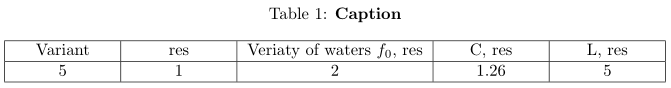
\includegraphics[width=1\linewidth]{4.5.png}
\textit{a command was also created to make a new cell view in the table}
}{4.4}
\end{minipage}
&
\begin{minipage}[m]{0.55\textwidth}
\renewcommand\textminus{\mbox{-}}%<<<<<<<<<<<
\begin{lstlisting}[numberstyle=\zebra{green!15}{yellow!15},numbers=left,basicstyle=\ttfamily\scriptsize]{tex}
\usepackage{graphicx}
\usepackage{tabularx}
\newcolumntype{Y}{>{\centering\arraybackslash}X}
\begin{document}
\begin{table}[h!]
\begin{center}
\caption{\textbf{Caption}}
  \begin{tabularx}{14cm}{|Y|Y|c|Y|Y|}
  \hline
  Variant & res & Veriaty of waters $f_0$, res & C, res & L, res\\
  \hline
  5       &     1   &               2               & 1.26 & 5\\
  \hline
  \end{tabularx}
\end{center}
\end{table}
\end{lstlisting}
\end{minipage}
\end{tabular}
\end{table}

%#################### 4.5 ####################
\section{Photo positioning}
\begin{tabular}{c | c}
\begin{minipage}[m]{0.4\textwidth}
\enum{
\begin{tcolorbox}[enhanced,sharp corners,
width={5cm},
colback=white,
overlay={\node at (frame.south east) {\includegraphics[scale=0.1]{example-image-a}};} ]
Sample text here.
\end{tcolorbox}}{4.5}
\end{minipage}
&
\begin{minipage}[m]{0.55\textwidth}
\renewcommand\textminus{\mbox{-}}%<<<<<<<<<<<
\begin{lstlisting}[numberstyle=\zebra{green!15}{yellow!15},numbers=left,basicstyle=\ttfamily\footnotesize]{tex}
\documentclass{article}
\usepackage[most]{tcolorbox}
\usepackage{graphicx}
\begin{document}
\begin{tcolorbox}[enhanced,sharp corners,
width={5cm},
colback=white,
overlay={\node at (frame.south east) {\includegraphics[scale=0.1]{example-image-a}};} ]
Sample text here.
\end{tcolorbox}
\end{document}  
\end{lstlisting}
\end{minipage}
\end{tabular}

\clearpage

%#################### 4.6 ####################
\section{bclogo – Creating colourful boxes with logos}
\begin{table}[h!]
\begin{tabular}{c | c}
\begin{minipage}[m]{0.4\textwidth}
\enum{\href{https://ctan.org/pkg/bclogo}{\img{1}{images/4.5/4.5.pdf}}}{4.6}
\end{minipage}
&
\begin{minipage}[m]{0.55\textwidth}
\renewcommand\textminus{\mbox{-}}%<<<<<<<<<<<
\begin{lstlisting}[numberstyle=\zebra{green!15}{yellow!15},numbers=left,basicstyle=\ttfamily\scriptsize]
\documentclass{article}
\usepackage{geometry}
\geometry{
paperwidth=8cm,
paperheight=14cm,
margin=0.5cm
}
\usepackage{xcolor}
\usepackage[most]{tcolorbox}
\usepackage[tikz]{bclogo}

\newtcolorbox{framedd}[1][]{
  colframe=lightgray,
  colback=yellow!40!white,
  enhanced jigsaw,
  sharp corners,
  lower separated=false,
  lefthand width=1cm,
  sidebyside gap=0.5cm,
  sidebyside,#1}

\begin{document}
\begin{framedd}
  \bcbombe  \tcblower  Some text inside.
\end{framedd}

\begin{framedd}[colback=blue!40!green]
  \bclampe   \tcblower  Some text inside.
\end{framedd} 

\begin{framedd}
  \bcattention  \bcinterdit  \tcblower
  Some text inside.
\end{framedd}

\begin{framedd}[colback=blue!40!green]
   \bcnucleaire  \tcblower
  Some text inside.
\end{framedd}

\begin{framedd}[colback=blue!40!green]
 \bcdanger \tcblower
  Some text inside.
\end{framedd}

\begin{framedd}
  \bcquestion \tcblower
  Some text inside.
\end{framedd}

\begin{framedd}[colback=blue!40!green, lefthand width=2.5cm]
  \bcsoleil  \bceclaircie \bcpluie  \bcneige \tcblower
  Some text inside.
\end{framedd}

\begin{framedd}[lefthand width=3cm]
  \bccube \bcdodecaedre \bcicosaedre \bcoctaedre \bctetraedre  \tcblower
  Some text inside.
\end{framedd}
\end{document}
\end{lstlisting}
\end{minipage}
\end{tabular}
\end{table}

  
\clearpage
%#################### 4.7 ####################
\section{Warning banner}
\begin{tabular}{c | c}
\begin{minipage}[m]{0.4\textwidth}
\enum{
\begin{caja}[title=warning]
Here is some text 
\end{caja}}{4.7}
\end{minipage}
&
\begin{minipage}[m]{0.55\textwidth}
\renewcommand\textminus{\mbox{-}}%<<<<<<<<<<<
\begin{lstlisting}[numberstyle=\zebra{green!15}{yellow!15},numbers=left,basicstyle=\ttfamily\footnotesize]{tex}
\usepackage[utf8]{inputenc}
\usepackage[T1]{fontenc}
\usepackage[most]{tcolorbox}
\definecolor{orang}{RGB}{255,155,0}
\newtcolorbox[auto counter,number within=section]{caja}[1][]{
enhanced jigsaw,colback=white,colframe=orang,coltitle=orang,
fonttitle=\bfseries\sffamily,
sharp corners,
detach title,
leftrule=10mm,
% What you need %%%%%%%%%%%%
underlay unbroken and first={\node[below,text=black,anchor=east]
at ([xshift=-5.5pt]interior.base west) {\Huge  \textbf{!}};},
%%%%%%%%%%%%%%%%%%%%%%%%
breakable,pad at break=1mm,
#1,
code={\ifdefempty{\tcbtitletext}{}{\tcbset{before upper={\tcbtitle\par\medskip}}}},}
\begin{document}
\begin{caja}[title=warning]
The vertical alignment settings 
\end{caja}
\end{document}	
\end{lstlisting}
\end{minipage}
\end{tabular}

\vspace{0.2cm}	

%#################### 4.8 ####################
\section{Absolutely centered cells (vertically and horisontally)}
\begin{tabular}{c | c}
\begin{minipage}[m]{0.4\textwidth}
\enum{

 
\makegapedcells
    \begin{tabular}{|c|c|c| }
    \hline
all&in&cells\\ \hline
are&centered&vertically\\ \hline
and&horisontally&$\sum$\\ \hline
 
\end{tabular}
 
 }{4.8}
\end{minipage}
&
\begin{minipage}[m]{0.55\textwidth}
\renewcommand\textminus{\mbox{-}}%<<<<<<<<<<<
\begin{lstlisting}[numberstyle=\zebra{green!15}{yellow!15},numbers=left,basicstyle=\ttfamily\footnotesize]{tex}
\documentclass{article}
\usepackage{float}
\usepackage{array, makecell}
\setcellgapes{5pt}

\begin{document}
\begin{table}[H]
\center
\makegapedcells
    \begin{tabular}{|c|c|c|c|}
    \hline
1&1&1&1\\ \hline
1&1&1&1\\ \hline
1&1&1&1\\ \hline
 
\end{tabular}
\end{table}

\end{document}
\end{lstlisting}
\end{minipage}
\end{tabular}

%#################### 4.9 ####################
\section{Martix made of table}
\begin{tabular}{c | c}

\begin{minipage}[m]{0.4\textwidth}
\enum{    
 
\begin{tabular}{l|l c r|l}
 
        & $a_{1,1}$ & $\dots, a_{1,n}$ & 0 &                 \\  
        & $a_{1,1}$ & $\dots, a_{1,n}$ & 0 &                 \\ 
        & \multicolumn{3}{l|}{\dotfill}   &                  \\  
        & $a_{1,1}$ & $\dots, a_{1,n}$ & 0 &                 \\ 
$d_{n+1}$ &         &                &   & = 0 \\  
        & $a_{1,1}$ & $\dots, a_{1,n}$ & 0 &                 \\  
        & $a_{1,1}$ & $\dots, a_{1,n}$ & 0 &                 \\ 
        & \multicolumn{3}{l|}{\dotfill}   &                  \\ 
        & $a_{1,1}$ & $\dots, a_{1,n}$ & 0 &                 \\ 
\end{tabular}
 }{4.9}

\end{minipage}
&
\begin{minipage}[m]{0.55\textwidth}
\renewcommand\textminus{\mbox{-}}%<<<<<<<<<<<
\begin{lstlisting}[numberstyle=\zebra{green!15}{yellow!15},numbers=left,basicstyle=\ttfamily\footnotesize]{tex}
\documentclass[a4paper,14pt]{extreport}
\begin{document}
\begin{table}[]
\begin{tabular}{l|l c r|l}
& $a_{1,1}$ & $\dots, a_{1,n}$ & 0 &                 \\  
& $a_{1,1}$ & $\dots, a_{1,n}$ & 0 &                 \\ 
& \multicolumn{3}{l|}{\dotfill}   &                  \\  
& $a_{1,1}$ & $\dots, a_{1,n}$ & 0 &                 \\ 
$d_{n+1}$ &         &    &   & = $\pm 2ad_n$ = 0     \\  
& $a_{1,1}$ & $\dots, a_{1,n}$ & 0 &                 \\  
& $a_{1,1}$ & $\dots, a_{1,n}$ & 0 &                 \\ 
& \multicolumn{3}{l|}{\dotfill}   &                  \\ 
& $a_{1,1}$ & $\dots, a_{1,n}$ & 0 &                 \\ 
\end{tabular}
\end{table}
\end{document}
\end{lstlisting}
\end{minipage}
\end{tabular}

%#################### 4.10 ####################
\section{Centering cells with \xmybox{NiceTabular}}
\begin{tabular}{c | c}
\begin{minipage}[m]{0.4\textwidth}
\enum{ \begin{NiceTabular}{|c|c|c|} 
\hline
\cellcolor{red}1& \cellcolor{green}1 & \cellcolor{black!10}EVERY\\\hline 
\cellcolor{orange}1 & \cellcolor{red!35}1 & \cellcolor{brown!50}CELL \\ \hline
\cellcolor{green!35}1 & \cellcolor{blue!45}1 & \cellcolor{yellow}CENTERED \\ \hline
\end{NiceTabular}  }{4.10}
\end{minipage}
&
\begin{minipage}[m]{0.55\textwidth}
\renewcommand\textminus{\mbox{-}}%<<<<<<<<<<<
\begin{lstlisting}[numberstyle=\zebra{green!15}{yellow!15},numbers=left,basicstyle=\ttfamily\footnotesize] 
\documentclass{article}
\usepackage[table]{xcolor}
\usepackage{nicematrix}
\NiceMatrixOptions{cell-space-top-limit=5pt,cell-space-bottom-limit=5pt}

\begin{document}
\begin{table}[htbp]
\centering
\begin{NiceTabular}{|c|c|c|} 
\hline
\cellcolor{red}1& \cellcolor{green}1 &  1 \\ \hline 
\cellcolor{orange}1 & \cellcolor{red!35}1 &  1 \\ \hline
\cellcolor{green!35}1 & \cellcolor{blue!45}1 &  1 \\ \hline
\end{NiceTabular}
\end{table}
\end{document}
\end{lstlisting}
\end{minipage}
\end{tabular}


%#################### 4.11 ####################
\section{Centered cells in \xmybox{longtable}}
\begin{tabular}{c | c}
\begin{minipage}[m]{0.4\textwidth}
\enum{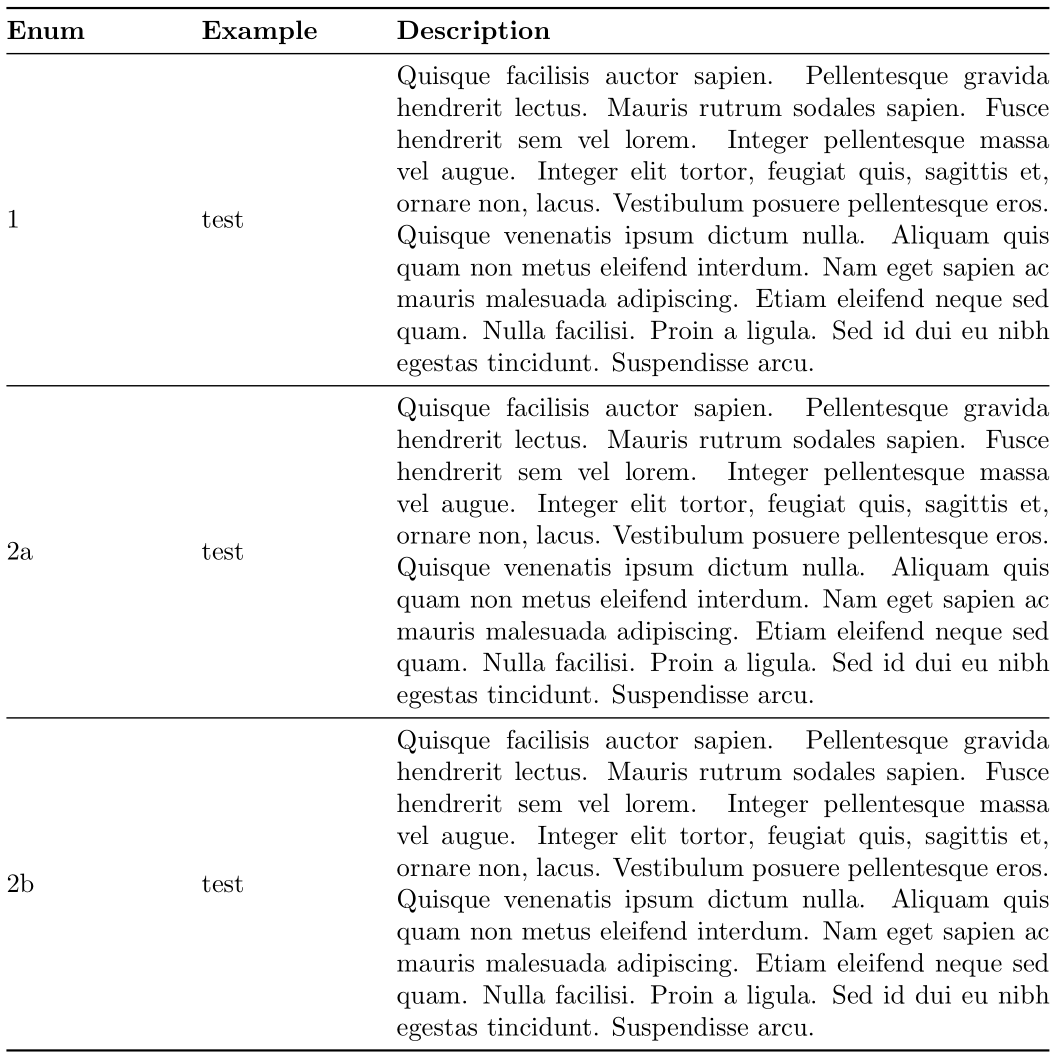
\includegraphics[width=1.\linewidth]{4.11.png}}{4.11}
\end{minipage}
&
\begin{minipage}[m]{0.55\textwidth}
\renewcommand\textminus{\mbox{-}}%<<<<<<<<<<<
\begin{lstlisting}[numberstyle=\zebra{green!15}{yellow!15},numbers=left,basicstyle=\ttfamily\scriptsize] 
\documentclass{article}
\usepackage[left=1.5cm,right=1.5cm,
top=1.5cm,bottom=2cm,bindingoffset=0cm]{geometry}
\usepackage{float}
\usepackage{array, makecell}
\usepackage[utf8]{inputenc}
\usepackage{lipsum}
\usepackage{booktabs}
\usepackage{multirow}
\usepackage{pdflscape}
\usepackage{longtable, array}

\begin{document}
\begin{landscape}
\begin{longtable}{@{} *{2}{m{.15\paperwidth}} *{1}{m{.40\paperwidth}} @{}}
\endfirsthead
\endhead
\toprule
\textbf{Enum} & \textbf{Example} & \textbf{Description} \\
\midrule
1 & test & \lipsum[50]\\
\midrule
2a & test & \lipsum[50]\\
2b & test & \lipsum[50]\\
\bottomrule
\end{longtable}
\end{landscape}
\end{document}          
\end{lstlisting}
\end{minipage}
\end{tabular}

%#################### 4.12 ####################
\section{If table is not wide enough}
\begin{tabular}{c | c}
\begin{minipage}[m]{0.4\textwidth}
\enum{ 
\begin{tabularx}{\textwidth}{X  X  X  X}
       & Item1 & Item2 & Item3 \\ \midrule
Group1 & 0.8   & 0.1   & 0.1  \\
Group2 & 0.1   & 0.8   & 0.1  \\
Group3 & 0.1   & 0.1   & 0.8  \\
Group4 & 0.34  & 0.33  & 0.33 \\ \bottomrule
\end{tabularx}}{4.12}
\end{minipage}
&
\begin{minipage}[m]{0.55\textwidth}
\renewcommand\textminus{\mbox{-}}%<<<<<<<<<<<
\begin{lstlisting}[numberstyle=\zebra{green!15}{yellow!15},numbers=left,basicstyle=\ttfamily\footnotesize] 
\documentclass{article}
\usepackage[left=1.5cm,right=1.5cm,
top=1.5cm,bottom=2cm,bindingoffset=0cm]{geometry}
\usepackage{graphicx}
\usepackage{booktabs}
\usepackage{tabularx}

\begin{document}         
\begin{table}[!ht] 
\caption{Vertical and lateral stresses of mortar.}  
\vspace{0.5cm}
\begin{tabularx}{\textwidth}{X  X  X  X}
       & Item1 & Item2 & Item3 \\ \midrule
Group1 & 0.8   & 0.1   & 0.1  \\
Group2 & 0.1   & 0.8   & 0.1  \\
Group3 & 0.1   & 0.1   & 0.8  \\
Group4 & 0.34  & 0.33  & 0.33 \\ \bottomrule
\end{tabularx}
\label{c}
\end{table}
\end{document}        
\end{lstlisting}
\end{minipage}
\end{tabular}


%#################### 4.13 ####################
\section{Text next to a table}
\begin{tabular}{c | c}
\begin{minipage}[m]{0.4\textwidth}
\enum{\begin{minipage}[m]{0.4\textwidth}
text  text text
\end{minipage}
\hfill
\begin{minipage}[m]{0.5\textwidth}
\begin{tabular}{|c|c|c|}
\hline
1 & 22 & 333  \\ \hline
  &    &      \\ \hline
  &    &      \\ \hline
  &    &      \\ \hline
\end{tabular}
\end{minipage}}{4.13}
\end{minipage}
&
\begin{minipage}[m]{0.55\textwidth}
\renewcommand\textminus{\mbox{-}}%<<<<<<<<<<<
\begin{lstlisting}[numberstyle=\zebra{green!15}{yellow!15},numbers=left,basicstyle=\ttfamily\footnotesize] 
\documentclass[a4paper,14pt]{extreport}
\usepackage[left=1.5cm,right=1.5cm,top=1.5cm,bottom=2cm,bindingoffset=0cm]{geometry}
\usepackage{lipsum}

\begin{document}
\begin{minipage}[m]{0.58\textwidth}
text text text
\end{minipage}
\hspace{0.2cm}
\begin{minipage}[m]{0.40\textwidth}
\begin{tabular}{|c|c|c|}
\hline
1 & 22 & 333 &  \\ \hline
  &    &     &  \\ \hline
  &    &     &  \\ \hline
  &    &     &  \\ \hline
\end{tabular}
\end{minipage}
\end{document}
\end{lstlisting}
\end{minipage}
\end{tabular}

%#################### 4.14 ####################
\section{Text next to a table}
\begin{tabular}{c | c}
\begin{minipage}[m]{0.4\textwidth}
\enum{  \center \begin{tikzpicture}[
    start chain=going below,
    node distance=2mm,
    Node/.style = {minimum width=#1,
                   shape=rectangle, 
                   draw, fill=white,
                   on chain},
    Pattern/.style = {pattern=north east hatch,
                    pattern color=teal!30,
                    hatch distance=7pt, 
                    hatch thickness=2pt},
    font=\small\sffamily]
%----------------
    \node[Node=24mm, Pattern, 
            preaction={fill=white}] (a) {without shadow};
    \begin{scope}[on background layer]
        \node[fit=(a),fill=red] {};
    \end{scope}

    \node[Node=24mm, drop shadow,
            preaction={fill=yellow}, Pattern] (b) {with shadow};

    \node[Node=24mm, preaction={fill=yellow},
            drop shadow, Pattern] (b) {with shadow};

    \node[Node=24mm, postaction={Pattern},
            drop shadow] (b) {with shadow};

    \node[Node=24mm, postaction={draw=red, Pattern},
            drop shadow] (b) {with shadow};

    \node[Node=24mm, drop shadow] (c) {without pattern};

   
%---
 \end{tikzpicture} 
  \href{https://tex.stackexchange.com/questions/154842/using-pattern-inside-tikz-shapes-with-dropped-shadows}{*****} }{4.14}
\end{minipage}
&
\begin{minipage}[m]{0.55\textwidth}
\renewcommand\textminus{\mbox{-}}%<<<<<<<<<<<
\begin{lstlisting}[numberstyle=\zebra{green!15}{yellow!15},numbers=left,basicstyle=\ttfamily\scriptsize] 
\documentclass[tikz,border=5mm]{standalone}
\usetikzlibrary{chains,patterns,shadows,fit,backgrounds}

\makeatletter
\tikzset{% customization of pattern
         % based on <m.wibrow@gm...> - 2013-03-24 07:20: 
        hatch distance/.store in=\hatchdistance,
        hatch distance=5pt,
        hatch thickness/.store in=\hatchthickness,
        hatch thickness=5pt
        }
\pgfdeclarepatternformonly[\hatchdistance,\hatchthickness]{north east hatch}% name
    {\pgfqpoint{-1pt}{-1pt}}% below left
    {\pgfqpoint{\hatchdistance}{\hatchdistance}}% above right
    {\pgfpoint{\hatchdistance-1pt}{\hatchdistance-1pt}}%
    {
        \pgfsetcolor{\tikz@pattern@color}
        \pgfsetlinewidth{\hatchthickness}
        \pgfpathmoveto{\pgfqpoint{0pt}{0pt}}
        \pgfpathlineto{\pgfqpoint{\hatchdistance}{\hatchdistance}}
        \pgfusepath{stroke}
    }
\makeatother

\begin{document}
 \begin{tikzpicture}[
    start chain=going below,
    node distance=2mm,
    Node/.style = {minimum width=#1,
                   shape=rectangle, 
                   draw, fill=white,
                   on chain},
    Pattern/.style = {pattern=north east hatch,
                    pattern color=teal!30,
                    hatch distance=7pt, 
                    hatch thickness=2pt},
    font=\small\sffamily]
%----------------
    \node[Node=24mm, Pattern, 
            preaction={fill=white}] (a) {without shadow};
    \begin{scope}[on background layer]
        \node[fit=(a),fill=red] {};
    \end{scope}

    \node[Node=24mm, drop shadow,
            preaction={fill=yellow}, Pattern] (b) {with shadow};

    \node[Node=24mm, preaction={fill=yellow},
            drop shadow, Pattern] (b) {with shadow};

    \node[Node=24mm, postaction={Pattern},
            drop shadow] (b) {with shadow};

    \node[Node=24mm, postaction={draw=red, Pattern},
            drop shadow] (b) {with shadow};

    \node[Node=24mm, drop shadow] (c) {without pattern};
%---
 \end{tikzpicture}   
\end{document}
\end{lstlisting}
\end{minipage}
\end{tabular}


%#################### 4.15 ####################
\section{Hand Drawn tcolorbox}
\begin{tabular}{c | c}
\begin{minipage}[m]{0.4\textwidth}
\enum{\begin{mytheo}{}{theoexample}
some text
\end{mytheo}}{4.15}
\end{minipage}
&
\begin{minipage}[m]{0.55\textwidth}
\renewcommand\textminus{\mbox{-}}%<<<<<<<<<<<
\begin{lstlisting}[numberstyle=\zebra{green!15}{yellow!15},numbers=left,basicstyle=\ttfamily\footnotesize] 
\documentclass{article}
\usepackage[most]{tcolorbox}
\usepackage{emerald}
\usetikzlibrary{decorations.pathmorphing}
\usetikzlibrary{shadows}
\tikzset{decoration={random steps,segment length=2mm,amplitude=0.6pt}}
\newtcbtheorem{mytheo}{Theorem}{
  coltitle=green!80!black,
  colback=lightgray!20,
  colbacktitle=lightgray!20,
  fonttitle=\bfseries\ECFAugie,
  enhanced,
  attach boxed title to top left={yshift=-0.18cm,xshift=-0.5mm},
  boxed title style={
    tikz={rotate=4,transform shape},
    frame code={
      \draw[decorate,fill=lightgray!20] (frame.south west) rectangle (frame.north east);
    }  },
  frame code={
    \draw[decorate,fill=lightgray!20,drop shadow] (frame.north east) rectangle (frame.south west);
  },}{th}

\begin{document}
\begin{mytheo}{}{theoexample}
content...
\end{mytheo}
\end{document}
\end{lstlisting}
\end{minipage}
\end{tabular}


%#################### 4.16 ####################%https://tex.stackexchange.com/questions/624558/how-can-i-do-this-block-in-beamer
\section{Halfframed boxes}
\begin{tabular}{c | c}
\begin{minipage}[m]{0.4\textwidth}
\enum{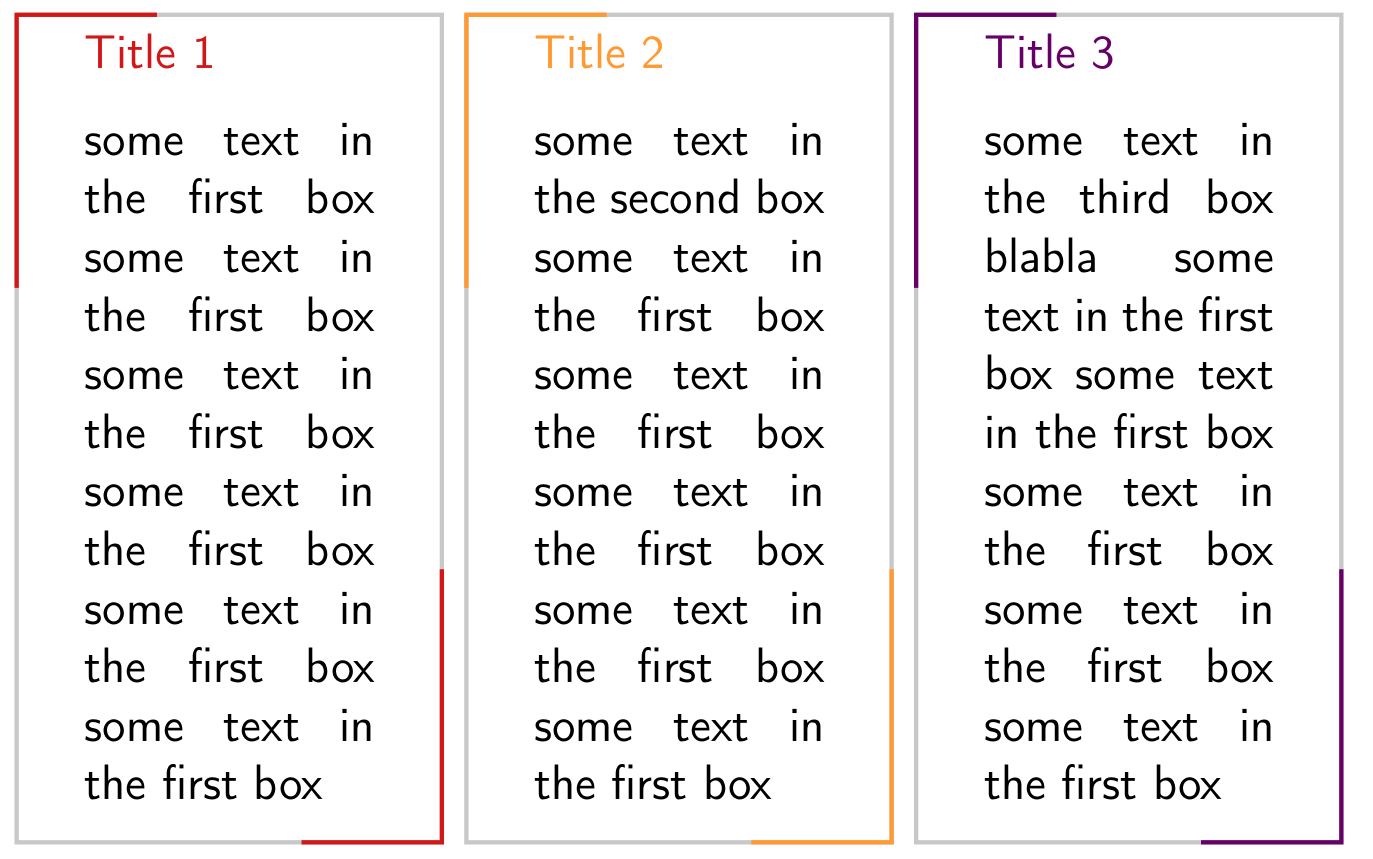
\includegraphics[width=1\linewidth]{4.16.png}}{4.16}
\end{minipage}
&
\begin{minipage}[m]{0.55\textwidth}
\renewcommand\textminus{\mbox{-}}%<<<<<<<<<<<
\begin{lstlisting}[numberstyle=\zebra{green!15}{yellow!15},numbers=left,basicstyle=\ttfamily\footnotesize] 
\documentclass{beamer}
\usepackage[english]{babel}
\usepackage[T1]{fontenc}
\usepackage[utf8]{inputenc}
\usepackage{tikz}
\usepackage{tcolorbox}
\usetikzlibrary{calc}
\tcbuselibrary{skins,breakable,raster}
\makeatletter
\definecolor{myred}{RGB}{209,23,23}
\definecolor{myorange}{RGB}{255,153,51}
\definecolor{mypurple}{RGB}{102,0,102}
\definecolor{mygrey}{RGB}{200,200,200}

\newtcolorbox{mybox}[2]{%
empty,
coltitle = #1,
title = #2,
overlay ={
\draw[mygrey,line width=1pt]
(frame.north west)--(frame.north east)--(frame.south east)--(frame.south west)--(frame.north west);
\draw[#1,line width=1pt]
($(frame.north west)!0.33!(frame.south west)$)
--(frame.north west)
--($(frame.north west)!0.33!(frame.north east)$);
\draw[#1,line width=1pt]
($(frame.south east)!0.33!(frame.south west)$)
--(frame.south east)
--($(frame.south east)!0.33!(frame.north east)$);}}

\tcbset{marktext/.style={%
  overlay={\node[rotate=90,text=black,anchor=north east] at (frame.north west){#1};},
  code={\setbox\z@=\color@hbox#1\color@endbox\tcbdimto\myheight{\wd\z@+3mm}},
  minimum for equal height group=\tcb@ehgid:\myheight,  }}
\makeatother

\begin{document}
\begin{frame}
\begin{tcbraster}[%
    raster columns=3,
    raster equal height=rows
    ]
    \begin{mybox}{myred}{Title 1}
    some text in the first box
    \end{mybox}
    \begin{mybox}{myorange}{Title 2}
    some text in the second box
    \end{mybox}
    \begin{mybox}{mypurple}{Title 3}
    some text in the third box blabla
    \end{mybox}
\end{tcbraster}
\end{frame}
\end{document}
\end{lstlisting}
\end{minipage}
\end{tabular}
%#################### 4.17 ####################
%#################### 4.18 ####################
%#################### 4.19 ####################










 
 